\documentclass[fontsize=12pt, a4paper]{scrartcl}
\let\stdsection\section 	% neue seite für neues kapitel
\renewcommand\section{\newpage\stdsection} 

% ### variables

\def \var_single_plot_width {0.49}
\def \var_double_plot_width {0.49}

% ### literaturverzeichnis
\usepackage[sorting=none]{biblatex}
\addbibresource{sim_axelsson.bib}

% ### sprachpakete
\usepackage[ngerman]{babel} % Deutsche Sprachanpassungen
\usepackage[T1]{fontenc}    % Silbentrennung bei Sonderzeichen
\usepackage[utf8]{inputenc} % Direkte Angabe von Umlauten im Dokument.
    
% ### grafiken   
\usepackage{graphicx}		% Zur Darstellung von Bildern
\usepackage{subcaption}
\usepackage{float}			% platziert figures am gewünschten platz
\usepackage[export]{adjustbox}% http://ctan.org/pkg/adjustbox

% ### matplotlib plots
\usepackage{pgf}
\usepackage{lmodern}% http://ctan.org/pkg/lm
%\usepackage{tikz}
\usepackage{pgfplots}
\pgfplotsset{width=10cm,compat=1.9}
%\pgfplotsset{compat=newest}

\usepackage{csquotes}

\usepackage[parfill]{parskip}

% ### curcuits
\usepackage{tikz}
\usetikzlibrary{arrows}
\usepackage[RPvoltages]{circuitikz}

% ### titleseite
\usepackage{titling}
\title{Systemmodelierung einer Membranpumpe für die Mikro-Fluidik}
\author{Kristjan Axelsson, Timo Stubler}
\date{\today}               

% ### fancy features
\usepackage{hyperref}

\begin{document}
\pagenumbering{gobble}		% turn off page numbers
\begin{titlingpage}
\begin{center}
\begin{figure}[H]
    \centering
    \begin{subfigure}[B]{0.2\textwidth}
        
\includegraphics[width=\textwidth, valign=t]{bilder/Logo_MNM_EN_Farbe_ohneHM (1).png}
    \end{subfigure}
    \begin{subfigure}[B]{0.45\textwidth}
        
\includegraphics[width=\textwidth, valign=t]{bilder/Hochschule_Muenchen_Logo.png}
    \end{subfigure}
\end{figure}
\setcounter{figure}{0}
\vspace{2cm}
\begin{large} 
\textbf{\thetitle} \\
\end{large}
\vspace{1cm}
\theauthor\\
\vspace{1cm}
Hochschule München \\
Fakultät für angewandte Wissenschaften und Mechatronik \\
\vspace{1cm}
\thedate
\end{center}
\end{titlingpage}

\tableofcontents            % Inhaltsverzeichnis anlegen

% quelle \cite{pedrotti} \\
% siehe Abb. \ref{fig_detector_test} \\
% siehe Kap. \ref{fazit}

\section{Einleitung}
\pagenumbering{arabic}		% turn on page numbers



\section{Theorie}

Im Folgenden wird die Modellierung der Membranpumpe besprochen. Der Antrieb der Pump wird durch einen Piezoaktor realisiert. Dieser wird über einen Wechselspannung betrieben und erzeugt so abwechselnd einen Über- bzw. Unterdruck in der Pumpkammer. Die Ventile sind passive Klappenventile welche nur in eine Richtung öffnen. Je nach Anordnung dient dieses Ventil einmal als Auslass und einmal als Einlass. Die Klappenventile sind über einen Schlauch jeweils mit einem Reservoir verbunden.

Im Folgenden werden zwei Modelle vorgestellt. Das erste Besteht aus der Pumpkammer mit einem Klappenventil und einer Zuleitung welche an eine Reservoir angeschlossen ist (einarmiges Model). Diese Model dient der Untersuchung der Ventile auf Leckströme und der Untersuchung der Zuleitungen auf deren Geometrie. Das zweite Model umfasst die Gesamte Pumpe welche auf ihre Funktionsweise bezogen auf Gegendruck und Antriebsfrequenz untersucht wird (zweiarmiges Model).

Für die Simulation wird ein fluidisches Ersatzmodel verwendet [Quelle Skript]

\[ Widerstand = Strömungswiderstand = \frac{m^3/s}{Pa} \]
\[ Kapazität = fluidische Kapazität = \frac{m^3}{Pa} \]
\[ Spannung = Druck = Pa \]

\[ P = R\dot{V} \]
\[ P = \frac{V}{C} \]
\[ P = P \]

\subsection{Reservoir}
Das Reservoir wird als unendlich groß angenommen und daher mit einem Konstanten Druck modelliert.


\[ Pr = Umgebungsdruck \]

Die Zuleitung wird durch einen einfachen Strömungswiderstand modelliert. Da diese Strömung als laminar betrachtet wird ist der Strömungswiderstand über das Gesetz von Hagen-Poiseuille zu beschreiben

\[ \dot{V} = \frac{pi * r^4 * dP}{8* eta *l} \]

\[ R = \frac{8* eta *l}{pi * r^4} \]

\subsection{Klappenventile}

Die Klappenventile werden durch einen Widerstand beschrieben welcher vom Druck abhängt. Für Drücke > 0 ist das Ventil geöffnent. Für Drücke < 0 ist das Ventil geschlossen. Die Widerstände für den geöffneten und geschlossenen Zustand werden über das oben beschriebene Gesetz von Hagen-Poiseuille beschrieben.

[Evtl. Grafik]

\subsection{Pumpkammer}
Real wird die Auslenkung der Pumpkammer durch Anlegen eines elektrischen Signales erzeugt. Dadurch verändert sich der Druck in der Pumpkammer, sowie dessen Kapazität. Die Pumpkammer ist in erster Näherung durch einen Kolben zu beschreiben. Die Höhe der Druckamplitude wird durch einen Proportionalitätsfaktor von der Spannung abhängig gemacht, ebenso die fluidische Kapazität. Die Extremwerte für Druck und Kapazität der Pumpkammer werden aus [Quelle ??] entnommen.

Die Trägheit der Pumpe wird über ein RC angenähert.

Der Wert für die Zeitkonstante wird abgeschätzt.

Hinterlegung der Kennlinie um in der Simulation zeitabhängige Werte für Pumpkammerdruck und -Kapazität zu bekommen.

[Kennlinien der Pumkammer]

\begin{figure}[H]
	\centering
	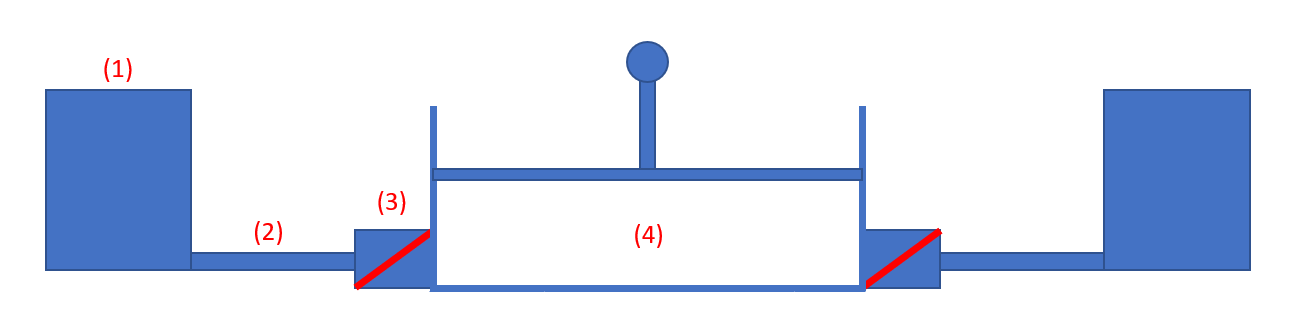
\includegraphics[width=0.98\textwidth]{bilder/theorie/pumpe_prinzipskizze.PNG}
	\caption{1) Reservoir 2) Zulauf 3) Ventil 4) Pumpkammer}
\end{figure}


\section{Modellierung}

Im Folgenden wird die Modellierung des einarmigen und zweiarmigen Models behandelt.

\subsection{Einarmig}

[Hier Ersatzschaltbild - Einarmig]

\[ Pin - Pt - Pv - Pc - Ps = 0 \]

\[ Pin - Rt\dot{V} - Rv(P)\dot{V} - \frac{V}{C(P)} - Ps(t) = 0 \]

\[ \dot{V} = \frac{Pin - Ps(t) - \frac{V}{C(P)}}{Rt - Rv(P)} \]


\subsection{Zweiarmig}

[Hier Ersatzschaltbild - Zweiarmig]

\section{Simulation}

Diese Kapitel umfasst die Untersuchungen des einarmigen und zweiarmigen Models der Membranpumpe

\subsection{Zuleitungen}

\begin{figure}[H]
	\centering
	\begin{subfigure}[H]{0.48\textwidth}
		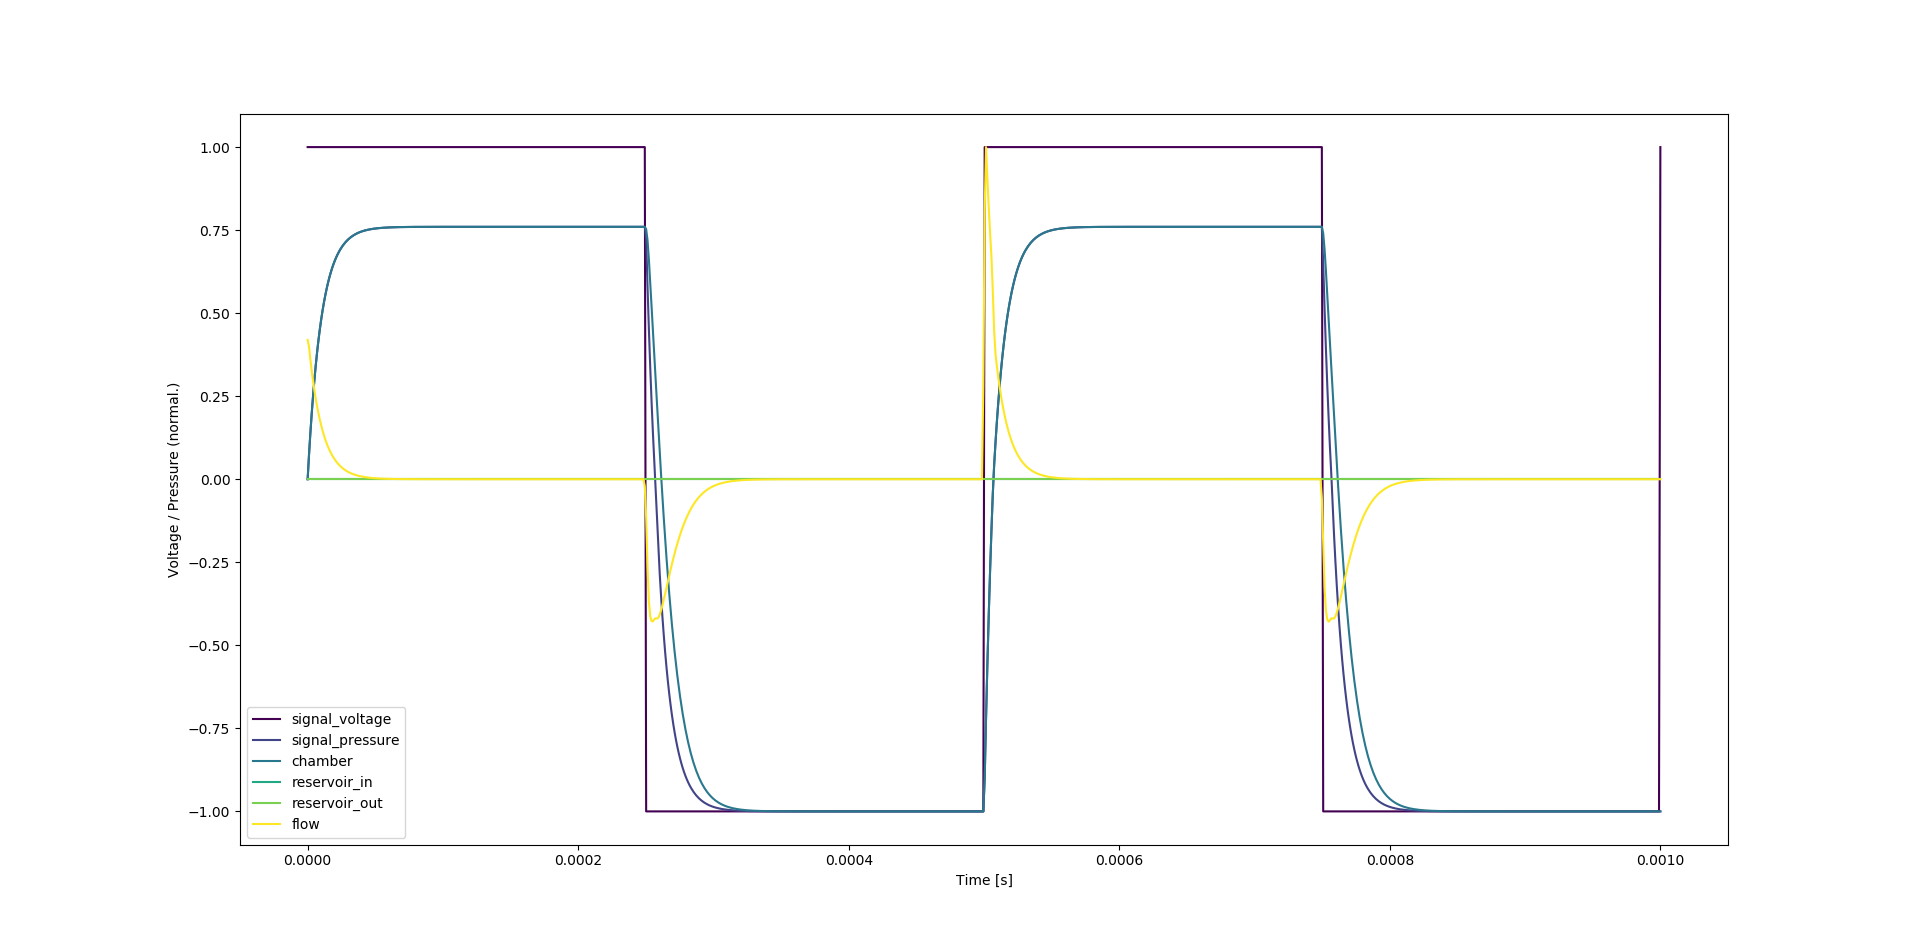
\includegraphics[width=\textwidth, valign=t]{bilder/tubelength/tl_in_branch_singlesweep.png}
		\caption{•}
	\end{subfigure}
	\begin{subfigure}[H]{0.48\textwidth}
		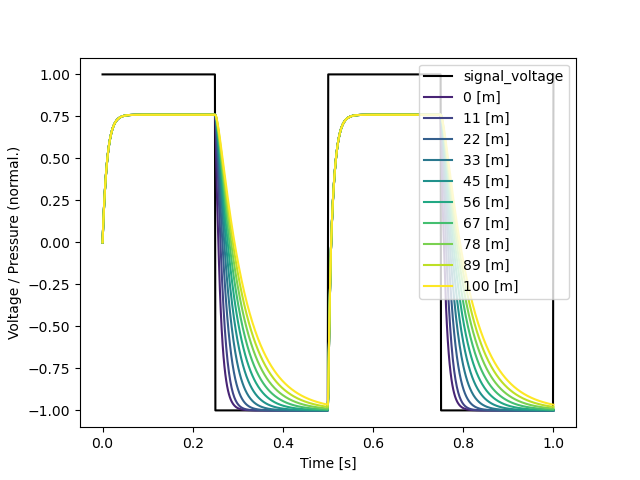
\includegraphics[width=\textwidth, valign=t]{bilder/tubelength/tl_in_branch_multisweep.png}
		\caption{•}
	\end{subfigure}
	\caption{•}
\end{figure}

\begin{figure}[H]
	\centering
	\begin{subfigure}[H]{0.48\textwidth}
		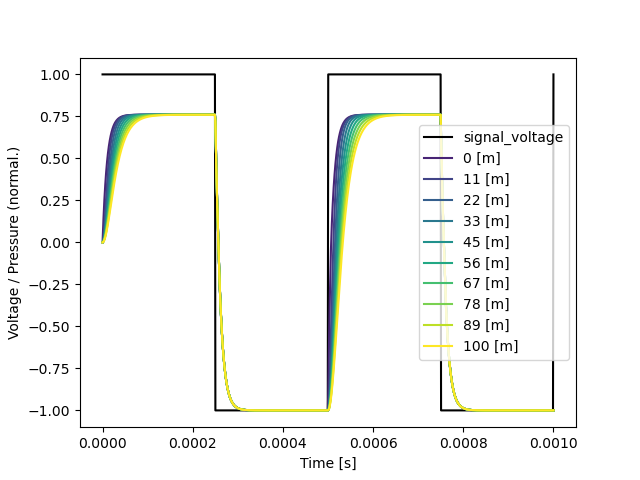
\includegraphics[width=\textwidth, valign=t]{bilder/tubelength/tl_out_branch_multisweep.png}
		\caption{•}
	\end{subfigure}
	\begin{subfigure}[H]{0.48\textwidth}
		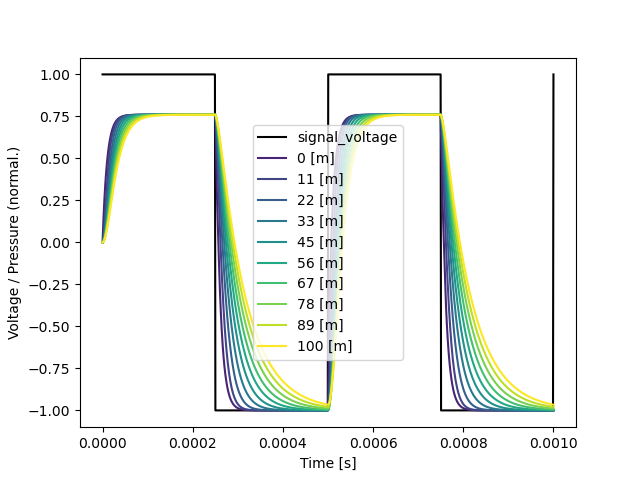
\includegraphics[width=\textwidth, valign=t]{bilder/tubelength/tl_both_branch_multisweep.png}
		\caption{•}
	\end{subfigure}
	\caption{•}
\end{figure}

\begin{figure}[H]
	\centering
	\begin{subfigure}[H]{0.4\textwidth}
		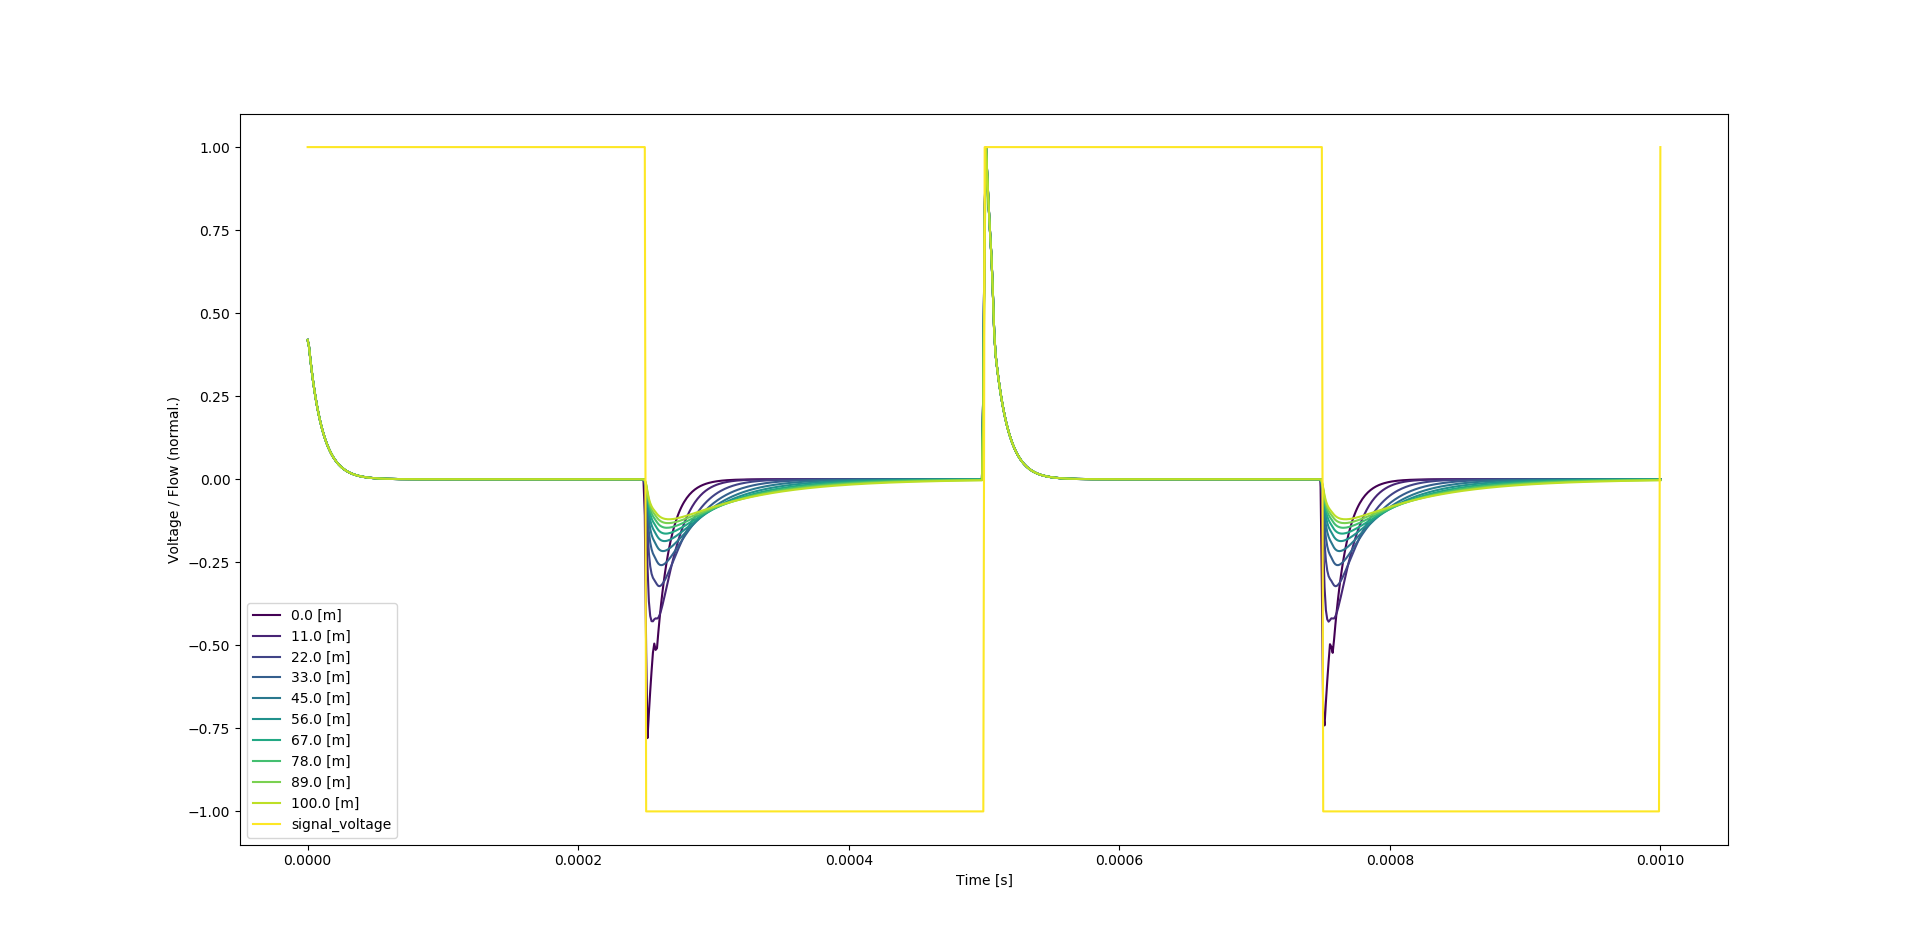
\includegraphics[width=\textwidth, valign=t]{bilder/tubelength/tl_in_branch_multisweep_flow.png}
		\caption{•}
	\end{subfigure}
	\begin{subfigure}[H]{0.48\textwidth}
	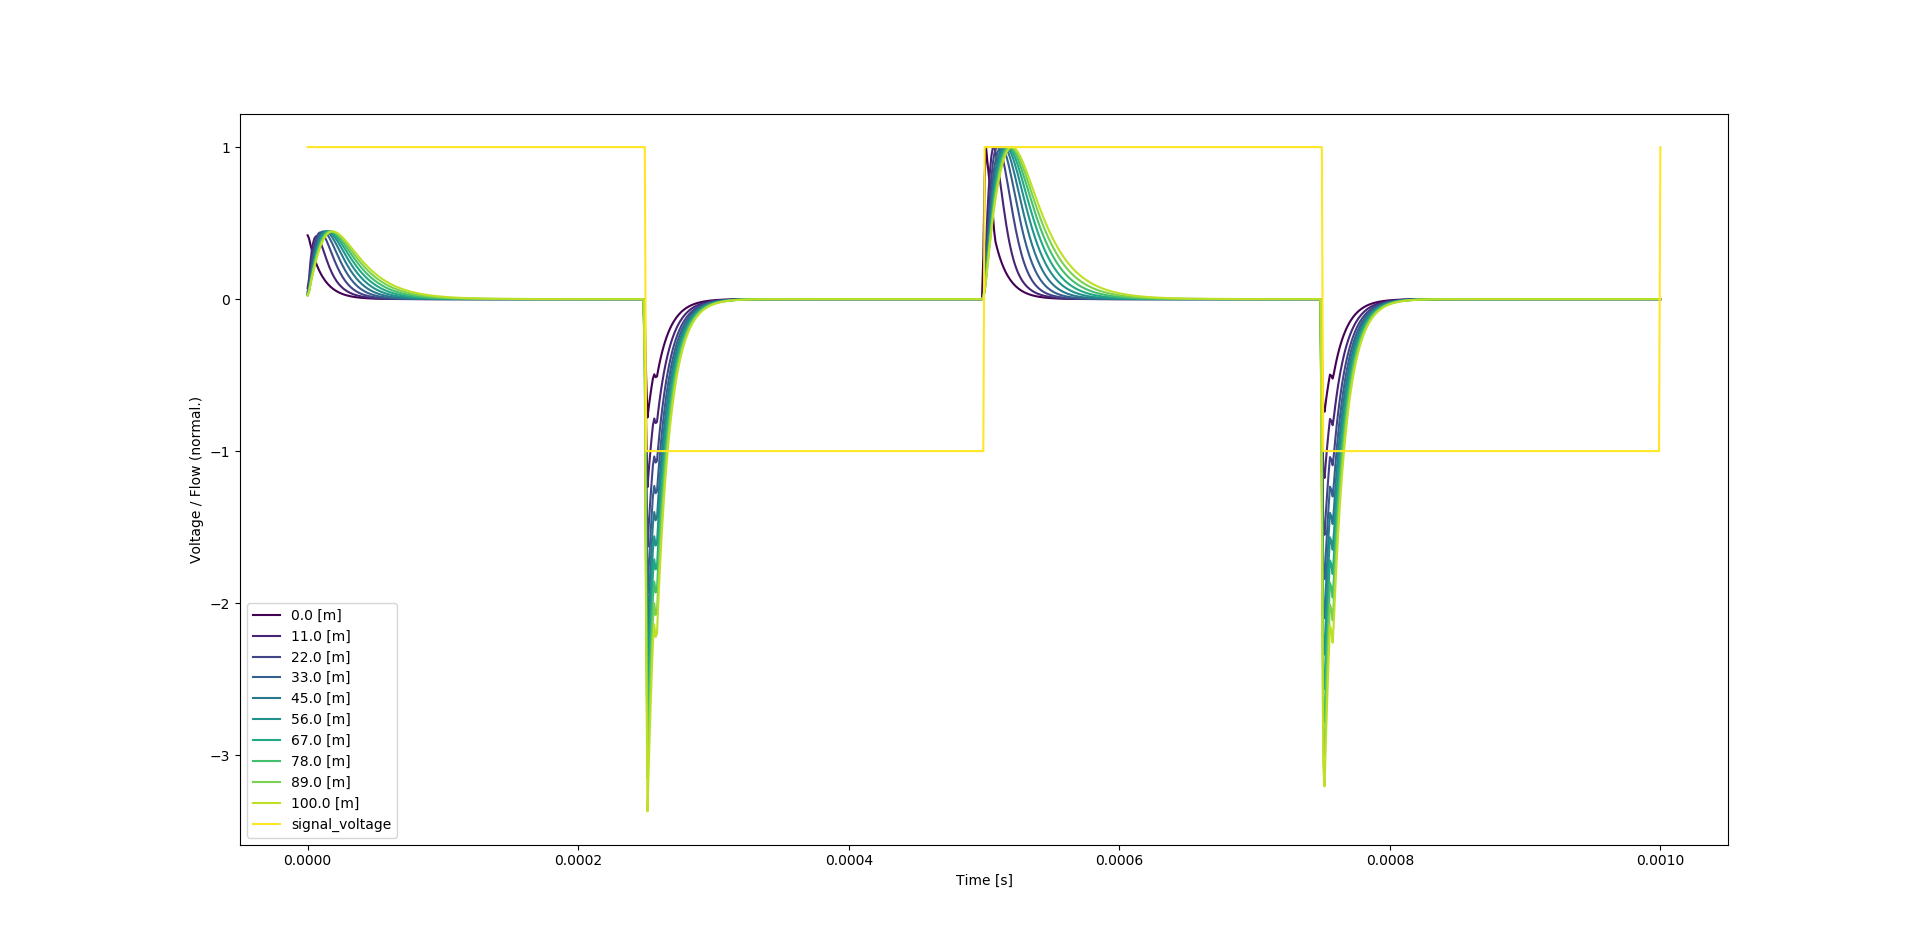
\includegraphics[width=\textwidth, valign=t]{bilder/tubelength/tl_out_branch_multisweep_flow.png}
	\caption{•}
	\end{subfigure}
	\begin{subfigure}[H]{0.48\textwidth}
		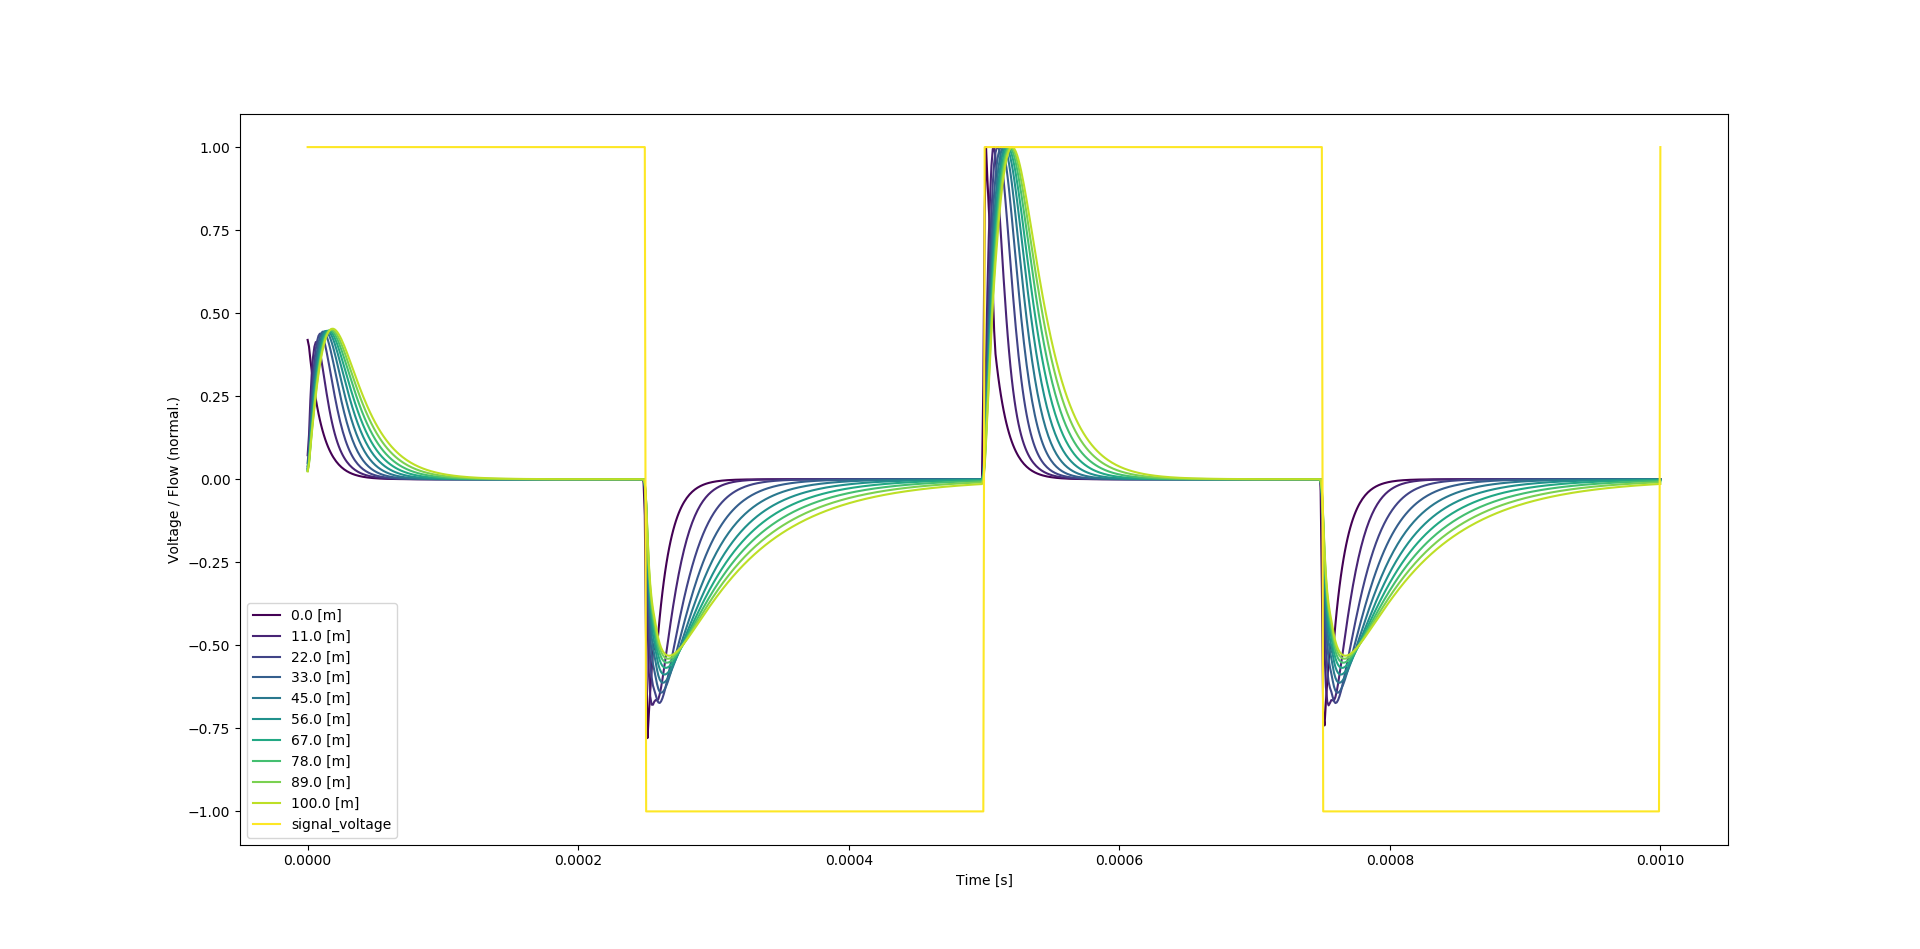
\includegraphics[width=\textwidth, valign=t]{bilder/tubelength/tl_both_branch_multisweep_flow.png}
		\caption{•}
	\end{subfigure}
	\caption{•}
\end{figure}

\subsection{Leckströme}

\begin{figure}[H]
	\centering
	\begin{subfigure}[H]{0.48\textwidth}
		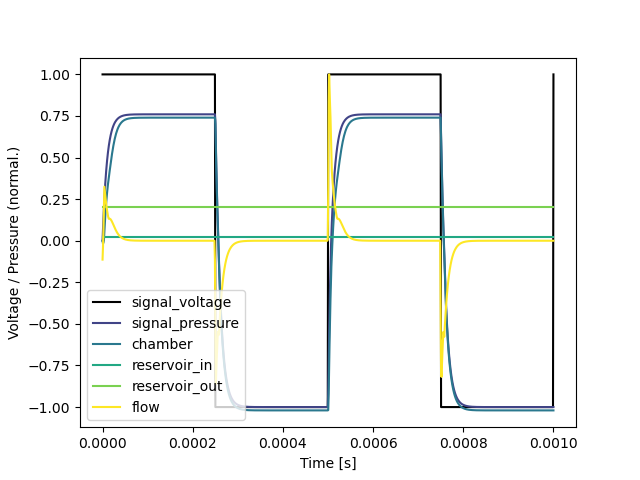
\includegraphics[width=\textwidth, valign=t]{bilder/velveresistance/vr_in_branch_singlesweep.png}
		\caption{•}
	\end{subfigure}
	\begin{subfigure}[H]{0.48\textwidth}
		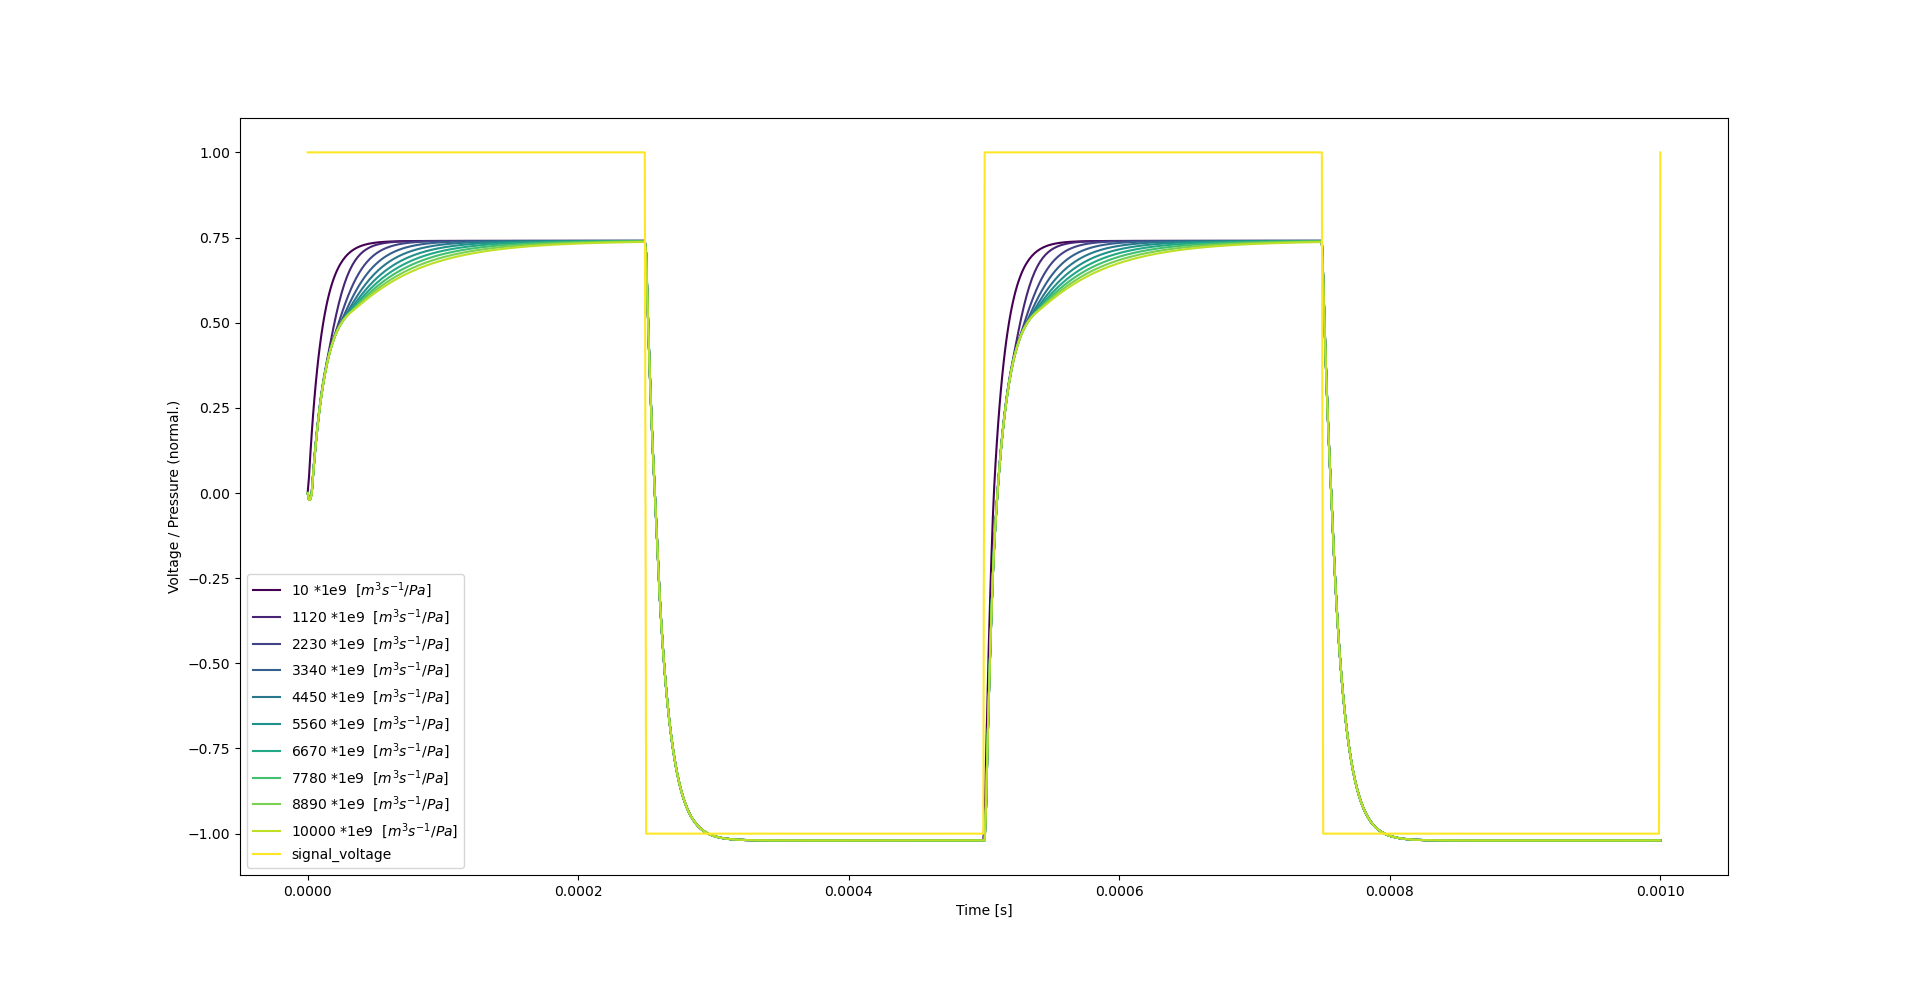
\includegraphics[width=\textwidth, valign=t]{bilder/velveresistance/vr_in_branch_multisweep.png}
		\caption{•}
	\end{subfigure}
	\caption{•}
\end{figure}

\begin{figure}[H]
	\centering
	\begin{subfigure}[H]{0.48\textwidth}
		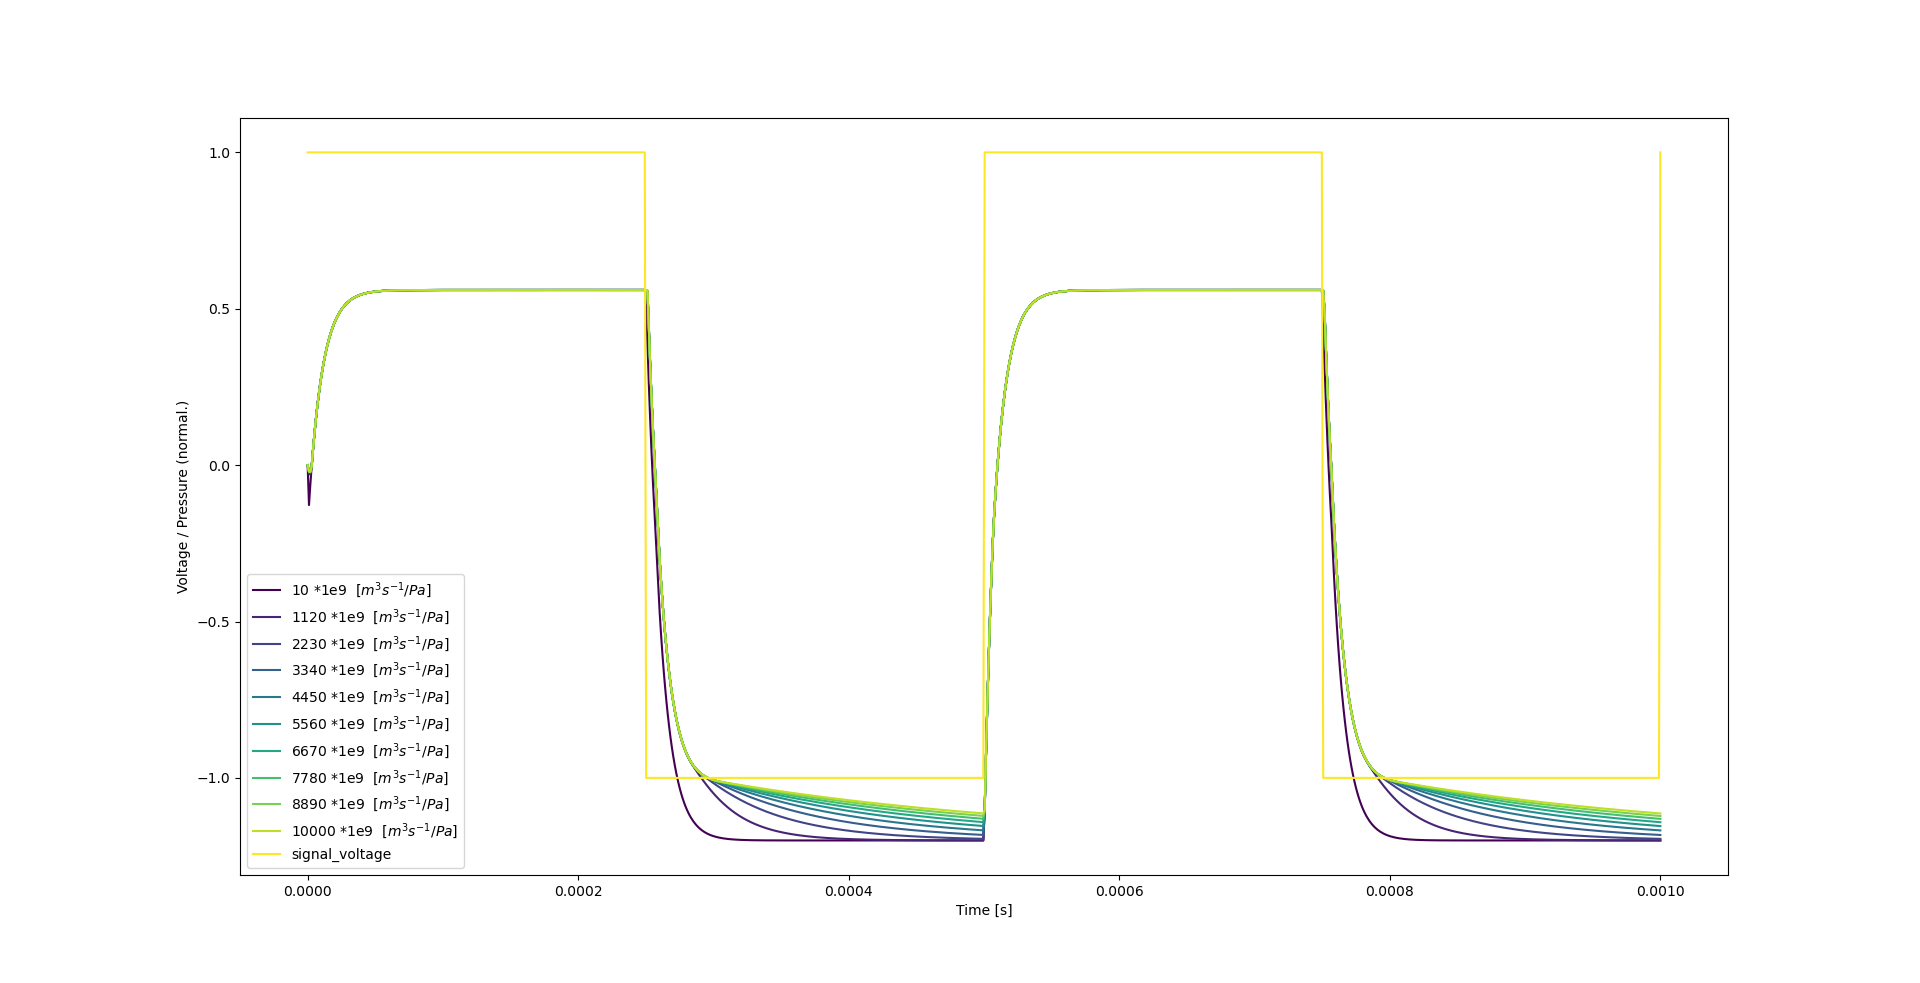
\includegraphics[width=\textwidth, valign=t]{bilder/velveresistance/vr_out_branch_multisweep.png}
		\caption{•}
	\end{subfigure}
	\begin{subfigure}[H]{0.48\textwidth}
		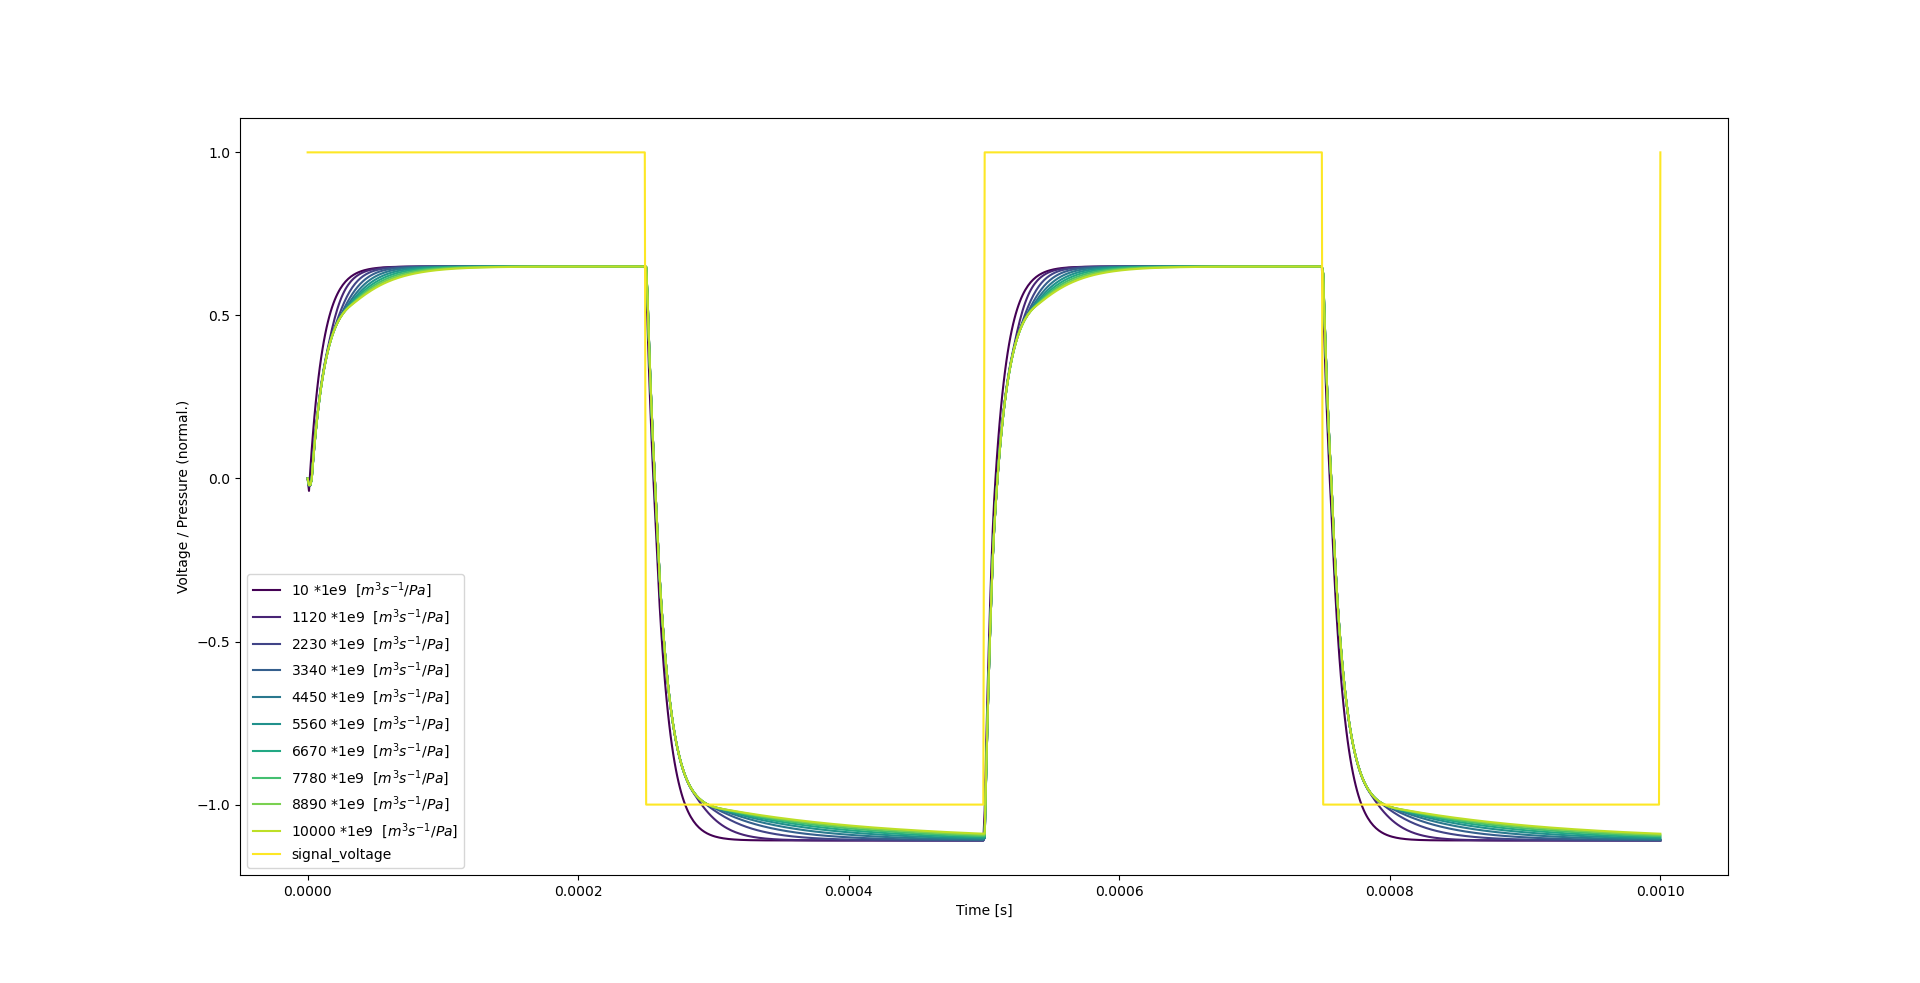
\includegraphics[width=\textwidth, valign=t]{bilder/velveresistance/vr_both_branch_multisweep.png}
		\caption{•}
	\end{subfigure}
	\caption{•}
\end{figure}

\subsection{Gegendruck}

\begin{figure}[H]
    \centering
    \begin{subfigure}[H]{0.48\textwidth}
        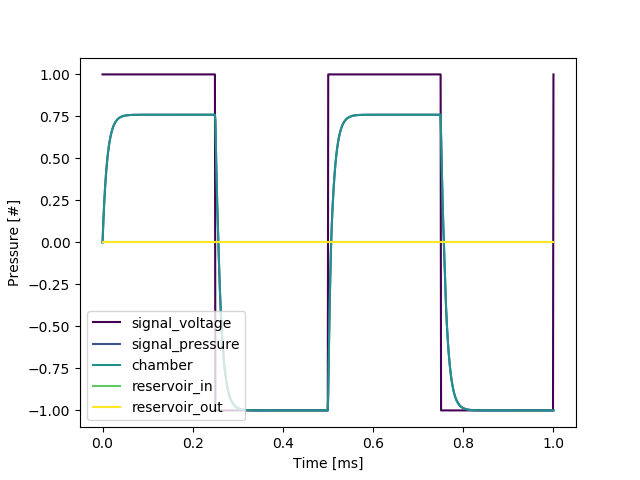
\includegraphics[width=\textwidth, valign=t]{bilder/backpressure/backpressure_free.png}
        \caption{•}
    \end{subfigure}
    \begin{subfigure}[H]{0.48\textwidth}
        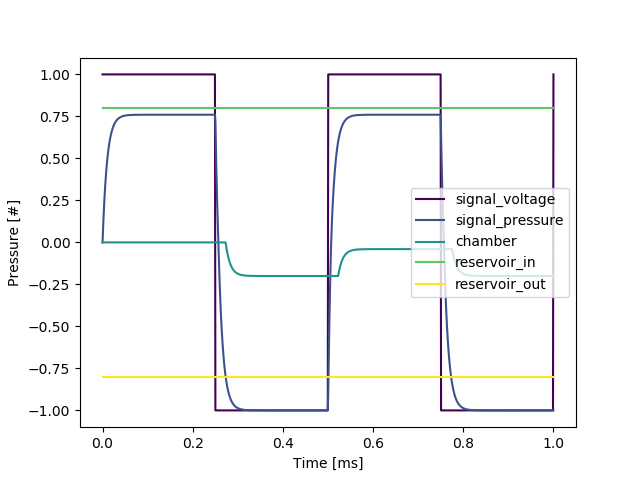
\includegraphics[width=\textwidth, valign=t]{bilder/backpressure/backpressure_example.png}
        \caption{•}
    \end{subfigure}
    \caption{•}
\end{figure}

\begin{figure}[H]
    \centering
    \begin{subfigure}[H]{0.48\textwidth}
        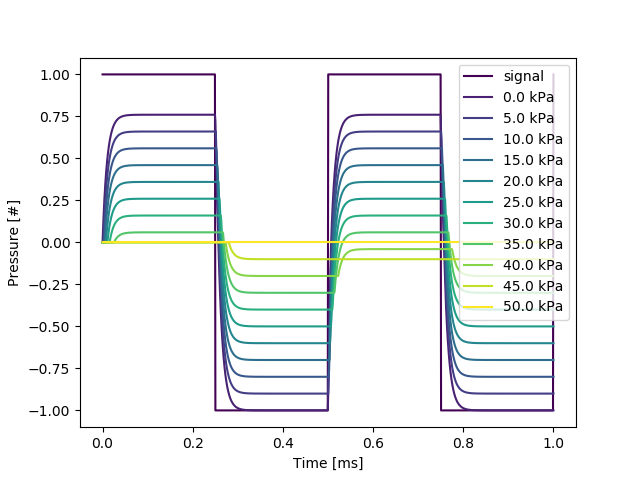
\includegraphics[width=\textwidth, valign=t]{bilder/backpressure/backpressure_at_pr_in_and_pr_out.png}
        \caption{•}
    \end{subfigure}
    \begin{subfigure}[H]{0.48\textwidth}
        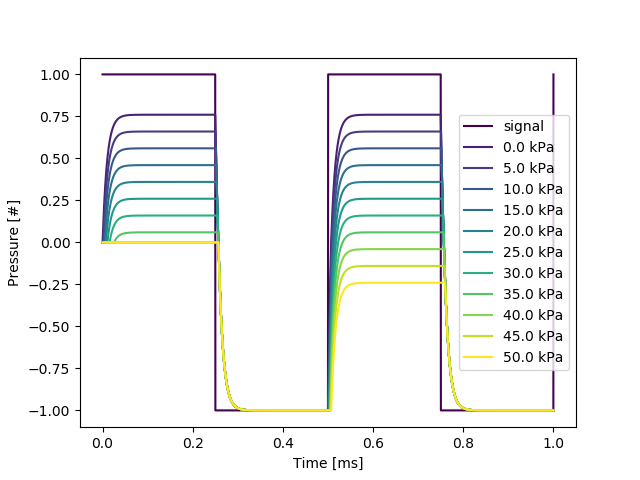
\includegraphics[width=\textwidth, valign=t]{bilder/backpressure/backpressure_at_pr_in.png}
        \caption{•}
    \end{subfigure}
    \caption{•}
\end{figure}

\begin{figure}[H]
	\centering
	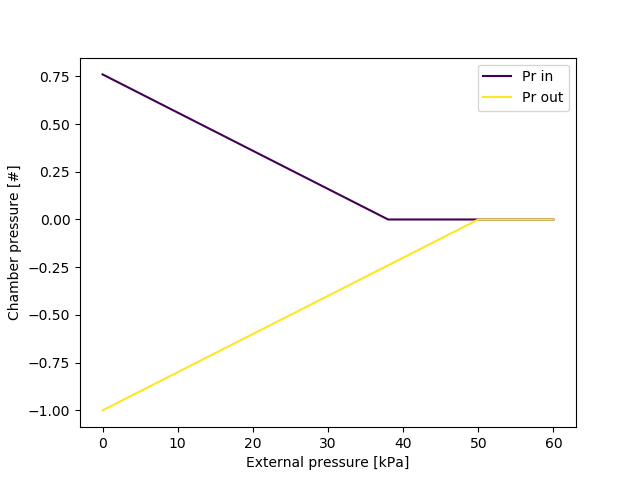
\includegraphics[width=0.7\textwidth]{bilder/backpressure/backpressure_result.png}
	\caption{•}
\end{figure}

\subsection{Grenzfrequenz}

\begin{figure}[H]
    \centering
    \begin{subfigure}[H]{0.48\textwidth}
        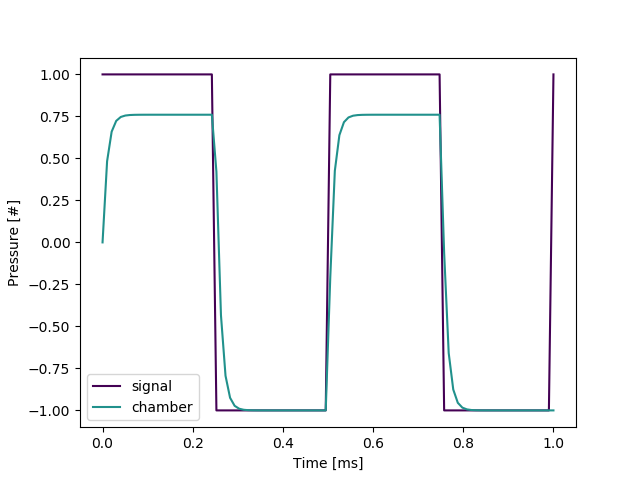
\includegraphics[width=\textwidth, valign=t]{bilder/frequency/frequency_default_2kHz.png}
        \caption{•}
    \end{subfigure}
    \begin{subfigure}[H]{0.48\textwidth}
        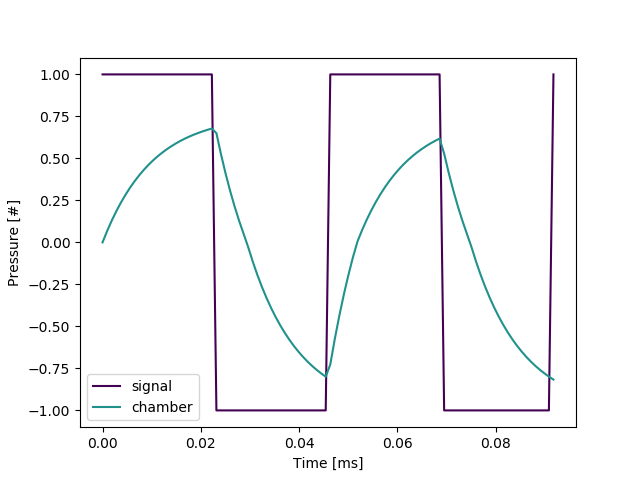
\includegraphics[width=\textwidth, valign=t]{bilder/frequency/frequency_to_fast_21_8 khz.png}
        \caption{•}
    \end{subfigure}
    \caption{•}
\end{figure}

\begin{figure}[H]
    \centering
    \begin{subfigure}[H]{0.48\textwidth}
        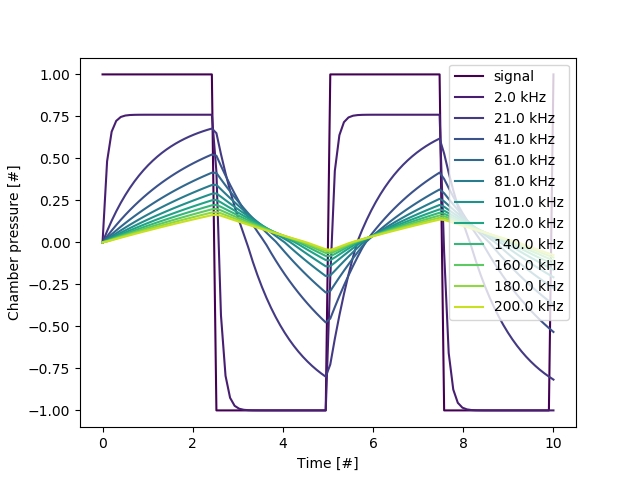
\includegraphics[width=\textwidth, valign=t]{bilder/frequency/frequency_sweep.png}
        \caption{•}
    \end{subfigure}
    \begin{subfigure}[H]{0.48\textwidth}
        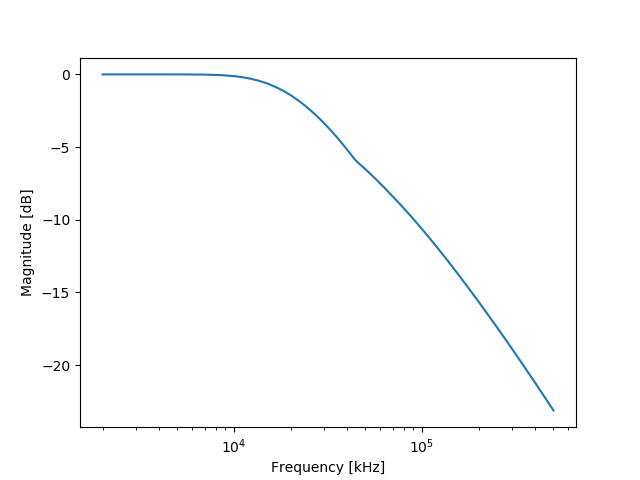
\includegraphics[width=\textwidth, valign=t]{bilder/frequency/bode_diagram.png}
        \caption{•}
    \end{subfigure}
    \caption{•}
\end{figure}

\section{Fazit}

\section{Ausblick}

\printbibliography

\end{document}
